\documentclass[../Main/Knit.tex]{subfiles}

% Plots
\iffalse
1.	Whole Transcriptome isoseq run output
2.	Rin correlation 
3.	CCS and FLNC reads, number of transcripts 
4.	Mapping alignment 
5.	Rarefaction curves
6.	Cage peaks 
7.	RNASeq 
8.	Isoforms across samples 
9.	ERCCs detected; correlation of ERCCs
10.	Isoform length
11.	Correlation of Isoforms with gene length 
12.	Correlation of Isoforms with exon number 
13.	RNASeq reads 
14.	Novel isoforms vs annotated; expression, length, exons 
15. CAGE,TSS,TTS peak novel vs annotated
16. AS events all, AS events independent events, 
17. Venn diagram of IR and NMD, low expression of IR and NMD 
18. LncRNA expression,transcript length and ORF 
\fi

% ONT comparisons
\iffalse
-	Comparing Read lengths 
-	Mappability 
-	Chimeric and gapped alignments 
-	Error patterns 
-	Isoform identification 
-	Isoform abundance estimation 

Sequencing quality (fraction of reads aligned) on read lengths for single pass reads (subreads for PacBio) and multi-pass consensus reads (CCS for PacBio and 2D reads for ONT) 
Fraction of Read aligned in bins

Context specific errors 

Pacbio non-size selection and Oxford Nanopore non-size selection
\fi

Lowly expressed gene and minor isoform quantification  
\section{Introduction}
 
\subsection{Mouse model of AD amyloidopathy: J20}
A mouse model of amyloidopathy, J20 overexpresses a mutant form human APP with two mutations identified by FAD, Indiana (V717F) and Swedish (K670N/M671L) mutations, directed by human platelet-growth-factor-beta promoter (PGRF-beta) with expression highest in the neocortex and hippocampus [Figure to show effects of mutations]. 
These mice exhibit defects in spatial memory and learning, with amyloid deposition by 5 – 7 moths, robust plaque formation by 8 – 10 months, and age-associated neuronal loss throughout the hippocampus. While J20 mouse closely resembles amyloidopathy development in human AD, insertion site of APP transgene has been shown to disrupt ZBTB20, a transcriptional repressor involved in hippocampal development.  

\subsection{Mouse model of AD tauopathy: rTg4510} 
Unlike with APP, there are currently no known mutations in MAPT linked to AD. Mouse models, such as rTG4510, that recapitulate AD tauopathy are therefore developed through harbouring missense mutations in MAPT that are associated with tauopathy in familial frontotemporal dementia (FTD). In the case with rTg4510, the human tau transgene carrying the P301L mutation is over-expressed under the calcium calmodulin kinase II promotor (CaMK2a) and is largely restricted to the forebrain (such as hippocampus and cortex). 
These mice also exhibit cognitive and behavioural impairments, with neurofibrillary tangles developing as early as 2 months, and associated neuronal and synaptic loss evident by 9 months. Starting from the neocortex and progressing rapidly to the hippocampus, the age-dependent spread of neuropathology in rTG4510 mouse closely reflects the spread of NFTs in human AD, as classified into Braak stages. However, it is important to note that the genomic integration of CAMK2a and MAPT transgene has been to have off-target effects with disruption in the endogenous mouse genes, including XXX. 
[Figure X: rTg4510 with image of why it is called regulatable due to the mouse line]


\newpage
\section{Methods}
As detailed in Chapter X, Pacific Biosciences Iso-Seq dataset was generated with whole transcriptome approach using high quality RNA from mouse cortex of rTg4510 model (n = 12, WT = 6, TG = 6, mean age = 5 months, range = 2 - 8 months) (Figure \ref{fig:isoseq_samples}). As a technological comparison and validation of the IsoSeq approach, a subset of samples were also sequenced on ONT (Figure \ref{fig:ONT_samples}). While both long-read sequencing approaches are superior to short-read RNA-Sequencing in the generation of full-length transcripts, there are major inherent batch biases due to the time-consuming and laborious protocol involved. The library preparation was standardised as much as possible, with the initial input of RNA for cDNA synthesis and the final library input for sequencing. However, due to the need for optimising each sample for library preparation and the rapid updates of sequencing chemistry throughout my PhD, each sample was effectively sequenced sequentially rather than as a batch [Figure X]. 

\subsection{RNA Extraction}
\label{section: ch2_rna_extraction}
Total RNA from mouse entorhinal cortex was extracted by Dr. Isabel Castanho using the AllPrep DNA/RNA Mini Kit (Qiagen). Samples were selected for long-read sequencing based on RNA quality and quantity, previously determined using RNA ScreenTape assay (Agilent) on 2200 TapeStation System or the RNA 6000 Nano kit (Agilent) on the 2100 Bioanalyzer (Section \ref{section:ch2_bioanalyzer}). 


Raw reads from each sample were processed using the Iso-Seq pipeline with optimised parameters (see Section X), with the aim to identify poly-A full-length transcripts by the presence of both primers and polyA tail, and the clustering of similar transcripts to generate a unique,consensus isoform, which is then annotated by mapping to a reference genome. Briefly, circular consensus reads (CCS) were generated from a minimum of 1 pass and RQ X. cDNA primers and SMRT adapters were then removed using Lima (v1.9) to generate full-length (FL) reads, followed by removal of artificial concatemers reads and trimming of polyA tails in Iso-Seq3 Refine. Full-length, non-concatemers (FLNC) reads were then collapsed, according to default parameters in Iso-Seq3 Cluster, to high-quality transcripts with accuracy $>$99\%, which were mapped to the reference mouse genome using minimap2 (v2.17). Transcripts were then further filtered based on mapping quality and clustered using Cupcake's collapse script, followed by SQANTI2 annotation to identify fusion transcripts, proximity to CAGE peaks derived from the FANTOM dataset, TSS and TTS sites and classification of lncRNA in combination with lcRNA gene annotation (vM22).  Subsequent filtering by TAMA was then applied to remove potential artifacts. CAGE peaks facilitates the mapping of transcripts, transcription factors, transcriptional promoters and enhancers. 

Alternative splicing events were assessed using a range of packages and custom scripts: mutually exclusive exons (MX) and skipped exons (SE) were assessed using SUPPA with the parameter –f ioe, intron retention (IR) with SQANTI2, and alternative first exons (AF), alternative last exons (AL), alternative 5’ splice sites (A5), and alternative 3’ splice sites (A3) using custom scripts based on splice junction coordinates. 

\iffalse
\newpage
\begin{figure}[h]
	\includegraphics[page=2, width=1\linewidth,height=0.4\textheight]{Pictures/IsoSeq_Samples.png}
	\captionsetup{width=0.95\textwidth}
	\caption[Tg4510 WT and TG samples sequenced using Whole and Targeted Iso-Seq]%
	{\textbf{Tg4510 WT and TG samples sequenced using Whole and Targeted Iso-Seq}: 12 samples at baseline and final age timepoint (WT = 6, TG = 6, ages = 2 months, 8 months) were sequenced using Whole Iso-Seq (highlighted boxes) and an additional 12 samples (WT = 6, TG = 6, ages = 4 months and 6 months) were sequenced using Targeted Iso-Seq (outlined). Text on each mouse figure refer to sample names}
	\label{fig:isoseq_samples}
\end{figure}

\begin{figure}[h]
	\includegraphics[page=2, width=1\linewidth,height=0.4\textheight]{Pictures/ONT_Samples.png}
	\captionsetup{width=0.95\textwidth}
	\caption[Tg4510 WT and TG samples sequenced using Whole and Targeted ONT]%
	{\textbf{Tg4510 WT and TG samples sequenced using Whole and Targeted ONT}: A subset of samples were also sequenced as whole transcriptome on ONT (WT = 1, TG = 1, age  = 2 months, highlighted boxes) and targeted on ONT (WT = 7, TG = 11, outlined). Text on each mouse figure refer to sample names}
	\label{fig:ONT_samples}
\end{figure}
\fi

\newpage
\section{Results}

12 mouse samples (6 WT and 6 TG) was sequenced using Iso-Seq approach on the PacBio Sequel 1 platform and analysed together for an accurate,deep characterisation of the full-length splice variants and identification of novel isoforms in the mouse transcriptome. 

\subsection{Run performance and sequencing metrics}
Following library preparation and single-molecule real time sequencing (SMRT), a total of 371Gb (s.d = 4.35Gb, range = 22.5Gb - 38.74Gb) and 8,082,647 polymerase reads (s.d = 63,013 reads, range = 530,974 - 733,495 reads) were obtained (Table \ref{tab:run_output}). No significant difference was reported between WT and TG (n = 12 animals, two-tailed unpaired t-test, t(10) = -0.636, P = 0.539,  Figure \ref{fig:isoseq_whole_run_output}a), and no significant correlation was observed between run yield and RIN across samples (n = 12 animals, Pearson's correlation, t = -0.98, df = 10, P = 0.350, Figure \ref{fig:isoseq_whole_run_output}b). Yield across all the samples are within the range as would expected from SMRT Iso-Seq library.   

%Check no difference between lengths CCS read lengths i.e. equal representation of RNA molecules; to make sure that we have a fair representation of reads of the RNA transcripts --> comparison of CCS reads and representation of RNA molecules between different base pairs lengths between different sample sets --> if fair representation, then expect log-ratio of interested sample/compared sample = - (10^0 =1)

\
\begin{table}[h]
	\begin{tabularx}{1\textwidth}{cccccc}
		\toprule
		Sample & Age      & Phenotype & RIN & Total Bases (GB) & Unique Yield (GB) \\ \midrule
		K17    & 2 months & WT   & 9.2 & 29.56            & -                           \\
		K18    & 2 months & TG   & 8.8 & 31.1             & 1.21                        \\
		K23    & 8 months & WT   & 9.1 & 34.60            & 2.06                        \\
		K24    & 8 months & TG   & 9.2 & 34.61            & 2.09                        \\
		L22    & 8 months & TG   & 8.7 & 38.74            & 2.1                         \\
		M21    & 2 months & WT   & 9.2 & 30.45            & -                           \\
		O18    & 2 months & TG   & 8.9 & 22.53            & 1.56                        \\
		O23    & 8 months & WT   & 9   & 31.25            & -                           \\
		Q20    & 8 months & TG   & 8.6 & 33.16            & 2.27                        \\
		Q21    & 2 months & WT   & 9.2 & 24.52            & 2.27                        \\
		S18    & 2 months & TG   & 8.9 & 30.41            & 1.69                        \\
		S23     & 8 months & WT   & 9.1 & 30.28            & -                          \\ \bottomrule
	\end{tabularx}
	\caption[Run Yield Output from Whole Transcriptome Iso-Seq of Tg4510]%
	{Phenotypic information and Iso-seq run yield for each sample of Tg4510 sequenced using Whole Transcriptome approach}
	\label{tab:run_output}
\end{table}

\begin{figure}[h]
	\begin{center}
	\includegraphics[page=1,trim={0 1cm 0 0},clip,scale = 0.55]{Pictures/WholeTranscriptome.pdf}
	\end{center}
	\captionsetup{width=0.95\textwidth}
	\caption[Whole Transcriptome Iso-Seq run yields and relationship to RIN score]%
	{\textbf{Whole Transcriptome Iso-Seq runs generated ~30Gb per sample, independent of RIN score}: Sequential Iso-Seq run generated \textbf{a)} a range of 30-35Gb per sample of the whole transcriptome, with no significant difference observed between WT and TG Tg4510 mice. Of note, two samples with $<$25Gb in WT and TG refer to earlier samples sequenced with a lower chemistry. \textbf{b)} Despite TG samples having distinctly lower RIN values than WT samples, no significant difference in yield output was observed between WT and TG.}
	\label{fig:isoseq_whole_run_output}
\end{figure}

\begin{landscape}
	\begin{table}[]
		\resizebox{1.5\textwidth}{!}{%
		\begin{tabular}{@{}cccccccccccccccccc@{}}
			\toprule
			\multirow{3}{*}{Sample} &
			\multirow{3}{*}{\begin{tabular}[c]{@{}c@{}}Polymerase\\ Reads\end{tabular}} &
			\multicolumn{6}{c}{Read   Length} &
			\multicolumn{3}{c}{Productivity} &
			\multicolumn{4}{c}{Control} &
			\multirow{3}{*}{\begin{tabular}[c]{@{}c@{}}Local\\  Base \\ Rate\end{tabular}} &
			\multicolumn{2}{c}{Template} \\ \cmidrule(lr){3-15} \cmidrule(l){17-18} 
			&
			&
			\multicolumn{2}{c|}{Polymerase} &
			\multicolumn{2}{c|}{Subread} &
			\multicolumn{2}{c|}{Insert} &
			\multicolumn{1}{c|}{\multirow{2}{*}{P0}} &
			\multicolumn{1}{c|}{\multirow{2}{*}{P1}} &
			\multicolumn{1}{c|}{\multirow{2}{*}{P2}} &
			\multicolumn{1}{c|}{\multirow{2}{*}{\begin{tabular}[c]{@{}c@{}}Total   \\ Reads\end{tabular}}} &
			\multicolumn{1}{c|}{\multirow{2}{*}{\begin{tabular}[c]{@{}c@{}}Pol RL  \\ Mean\end{tabular}}} &
			\multicolumn{2}{c|}{Concordance} &
			&
			\multicolumn{1}{c|}{\multirow{2}{*}{\begin{tabular}[c]{@{}c@{}}Adapter   \\ Dimer \\ (0-10bp)\end{tabular}}} &
			\multicolumn{1}{c|}{\multirow{2}{*}{\begin{tabular}[c]{@{}c@{}}Short\\  Insert\\  (11- 100bp)\end{tabular}}} \\ \cmidrule(lr){3-8} \cmidrule(lr){14-15}
			&
			&
			\multicolumn{1}{c|}{Mean} &
			\multicolumn{1}{c|}{N50} &
			\multicolumn{1}{c|}{Mean} &
			\multicolumn{1}{c|}{N50} &
			\multicolumn{1}{c|}{Mean} &
			\multicolumn{1}{c|}{N50} &
			\multicolumn{1}{c|}{} &
			\multicolumn{1}{c|}{} &
			\multicolumn{1}{c|}{} &
			\multicolumn{1}{c|}{} &
			\multicolumn{1}{c|}{} &
			\multicolumn{1}{c|}{Mean} &
			\multicolumn{1}{c|}{Mode} &
			&
			\multicolumn{1}{c|}{} &
			\multicolumn{1}{c|}{} \\ \midrule
			B21 &
			735598 &
			39971 &
			82100 &
			1531 &
			2125 &
			3162 &
			3896 &
			\begin{tabular}[c]{@{}c@{}}8.71\% \\ (87817)\end{tabular} &
			\begin{tabular}[c]{@{}c@{}}73.94\% \\ (745646)\end{tabular} &
			\begin{tabular}[c]{@{}c@{}}18.33\% \\ (184883)\end{tabular} &
			9940 &
			34144 &
			0.85 &
			0.89 &
			2.61 &
			0 &
			0 \\
			C20 &
			749931 &
			45670 &
			91153 &
			1426 &
			2066 &
			3204 &
			4075 &
			\begin{tabular}[c]{@{}c@{}}10.68\% \\ (107699)\end{tabular} &
			\begin{tabular}[c]{@{}c@{}}75.36\% \\ (759912)\end{tabular} &
			\begin{tabular}[c]{@{}c@{}}14.95\% \\ (150735)\end{tabular} &
			9910 &
			37019 &
			0.85 &
			0.89 &
			2.75 &
			0 &
			0 \\
			C21 &
			530395 &
			44208 &
			87750 &
			2258 &
			2794 &
			3358 &
			4250 &
			\begin{tabular}[c]{@{}c@{}}38.0\% \\ (387661)\end{tabular} &
			\begin{tabular}[c]{@{}c@{}}52.5\% \\ (535299)\end{tabular} &
			\begin{tabular}[c]{@{}c@{}}9.4\% \\ (96275)\end{tabular} &
			4880 &
			50690 &
			0.85 &
			0.85 &
			2.07 &
			0.00 &
			0.01 \\
			E18 &
			545,272 &
			41,036 &
			83,295 &
			2,467 &
			3,049 &
			3,588 &
			4,335 &
			\begin{tabular}[c]{@{}c@{}}38.88\% \\ (396026)\end{tabular} &
			\begin{tabular}[c]{@{}c@{}}53.61\% \\ (546027)\end{tabular} &
			\begin{tabular}[c]{@{}c@{}}7.58\% \\ (77181)\end{tabular} &
			722 &
			48,253 &
			0.85 &
			0.85 &
			2 &
			0 &
			0 \\
			K17 &
			673972 &
			43856 &
			90561 &
			1253 &
			2021 &
			3336 &
			4753 &
			\begin{tabular}[c]{@{}c@{}}10.55\% \\ (106,736)\end{tabular} &
			\begin{tabular}[c]{@{}c@{}}67.42\% \\ (681,794)\end{tabular} &
			\begin{tabular}[c]{@{}c@{}}22.73\% \\ (229,816)\end{tabular} &
			7036 &
			34651 &
			0.85 &
			0.89 &
			2.72 &
			0.08 &
			0.06 \\
			K18 &
			566086 &
			54892 &
			101220 &
			1256 &
			1775 &
			2863 &
			3661 &
			\begin{tabular}[c]{@{}c@{}}29.77\%\\ (299933)\end{tabular} &
			\begin{tabular}[c]{@{}c@{}}57.25\% \\ (576863)\end{tabular} &
			\begin{tabular}[c]{@{}c@{}}14.05\% \\ (141550)\end{tabular} &
			10707 &
			44640 &
			0.87 &
			0.89 &
			3.05 &
			0 &
			0 \\
			K23 &
			698178 &
			49563 &
			98801 &
			1697 &
			2670 &
			3779 &
			4779 &
			\begin{tabular}[c]{@{}c@{}}16.1\% \\ (164308)\end{tabular} &
			\begin{tabular}[c]{@{}c@{}}69.2\%  \\ (704197)\end{tabular} &
			\begin{tabular}[c]{@{}c@{}}14.7\%   \\ (149841)\end{tabular} &
			5951 &
			40498 &
			0.85 &
			0.89 &
			2.78 &
			0 &
			0 \\
			K24 &
			711015 &
			48675 &
			97024 &
			1714 &
			2487 &
			3834 &
			5018 &
			\begin{tabular}[c]{@{}c@{}}14.22\% \\ (144813)\end{tabular} &
			\begin{tabular}[c]{@{}c@{}}70.49\%\\  (717880)\end{tabular} &
			\begin{tabular}[c]{@{}c@{}}15.28\% \\ (155653)\end{tabular} &
			6762 &
			38363 &
			0.85 &
			0.87 &
			2.671 &
			0.01 &
			0.01 \\
			L22 &
			675283 &
			57370 &
			112630 &
			1869 &
			2867 &
			3903 &
			4793 &
			\begin{tabular}[c]{@{}c@{}}17.41\%\\ (175439 )\end{tabular} &
			\begin{tabular}[c]{@{}c@{}}68.08\%\\ (686007)\end{tabular} &
			\begin{tabular}[c]{@{}c@{}}15.58\% \\ (156900)\end{tabular} &
			10647 &
			44215 &
			0.86 &
			0.89 &
			2.96 &
			0.01 &
			0 \\
			M21 &
			660841 &
			46082 &
			91628 &
			2234 &
			2754 &
			3952 &
			4733 &
			\begin{tabular}[c]{@{}c@{}}16.6\%\\ (168567)\end{tabular} &
			\begin{tabular}[c]{@{}c@{}}65.9\%  \\ (671224)\end{tabular} &
			\begin{tabular}[c]{@{}c@{}}17.5\% \\  (178555)\end{tabular} &
			10301 &
			38690 &
			0.85 &
			0.87 &
			2.79 &
			0.01 &
			0.01 \\
			O18 &
			530974 &
			42423 &
			85331 &
			2609 &
			3146 &
			3443 &
			4082 &
			\begin{tabular}[c]{@{}c@{}}41.8\% \\  (426378\end{tabular} &
			\begin{tabular}[c]{@{}c@{}}52.6\%\\  (536435)\end{tabular} &
			\begin{tabular}[c]{@{}c@{}}5.5\% \\ (56422)\end{tabular} &
			5415 &
			49778 &
			0.86 &
			0.85 &
			2.05 &
			0 &
			0 \\
			O23 &
			730733 &
			42771 &
			89372 &
			1490 &
			2347 &
			3608 &
			4878 &
			\begin{tabular}[c]{@{}c@{}}9.37\% \\ (94536)\end{tabular} &
			\begin{tabular}[c]{@{}c@{}}73.33\% \\ (740184)\end{tabular} &
			\begin{tabular}[c]{@{}c@{}}18.19\% \\ (183626)\end{tabular} &
			8908 &
			34993 &
			0.85 &
			0.89 &
			2.56 &
			0.06 &
			0.04 \\
			Q20 &
			715206 &
			46360 &
			92519 &
			1,999 &
			2,926 &
			3,978 &
			4,954 &
			\begin{tabular}[c]{@{}c@{}}11.51\%\\  (117223)\end{tabular} &
			\begin{tabular}[c]{@{}c@{}}70.91\% \\ (722135)\end{tabular} &
			\begin{tabular}[c]{@{}c@{}}17.58\%\\  (178988)\end{tabular} &
			6855 &
			37990 &
			0.85 &
			0.87 &
			2.6 &
			0.01 &
			0.01 \\
			Q21 &
			733495 &
			33429 &
			70750 &
			2563 &
			3286 &
			3710 &
			4750 &
			\begin{tabular}[c]{@{}c@{}}15.9\% \\ (161679)\end{tabular} &
			\begin{tabular}[c]{@{}c@{}}72.1\%\\  (735250)\end{tabular} &
			\begin{tabular}[c]{@{}c@{}}12.0\% \\ (122305)\end{tabular} &
			1668 &
			44201 &
			0.85 &
			0.85 &
			1.99 &
			0.00 &
			0.01 \\
			S18 &
			682529 &
			44549 &
			90041 &
			1435 &
			2041 &
			3282 &
			4400 &
			\begin{tabular}[c]{@{}c@{}}11.98\%\\  (121,055)\end{tabular} &
			\begin{tabular}[c]{@{}c@{}}68.45\% \\ (691651)\end{tabular} &
			\begin{tabular}[c]{@{}c@{}}20.35\%\\  (205,640)\end{tabular} &
			7881 &
			36541 &
			0.86 &
			0.89 &
			2.85 &
			0.11 &
			0.07 \\
			S23 &
			704335 &
			42991 &
			89160 &
			1346 &
			2020 &
			3272 &
			4383 &
			\begin{tabular}[c]{@{}c@{}}7.02\%\\  (71074)\end{tabular} &
			\begin{tabular}[c]{@{}c@{}}70.18\% \\ (710471)\end{tabular} &
			\begin{tabular}[c]{@{}c@{}}23.39\% \\ (236801)\end{tabular} &
			6019 &
			35167 &
			0.85 &
			0.89 &
			2.57 &
			0.01 &
			0.01 \\ \bottomrule
		\end{tabular}%
	}
	\end{table}
\end{landscape}

With the application of long-reads bioinformatics pipeline (as detailed in Section X), the raw reads were processed and clustered to unique consensus transcripts, which were then mapped and annotated as isoforms - low-quality, lowly-supported, unmapped and degraded reads were sequentially filtered at each stage. Across all 12 samples, a total of 5.66M CCS reads (mean = 471K,s.d = 46.8K, range =  353K - 512K) and 4.55 FLNC reads were successfully generated (mean = 379K, s.d = 47.0K, range = 270K - 412K) after multiple processing (Figure \ref{fig:isoseq_whole_processing}a). Clustering of these reads yielded a total of 273K high-quality full-length transcripts (97\% of all FL transcripts, mean = 32.7K, s.d = 1.25K, range = 30.3K - 34.4K) (Figure \ref{fig:isoseq_whole_processing}b), and were mapped to 278K and 352 loci of the mouse reference (5K had multi-mapping) and ERCC annotations respectively. After filtering for 85\% alignment identity and 95\% length (Figure \ref{fig:isoseq_whole_processing}c), 266K transcripts were retained. No difference was observed in the number of transcripts generated between WT and TG (n = 12, two-tailed unpaired t-test, t = -0.005, df = 10, P = 0.996) or by age (n = 12, t = -1.58, df = 10, P = 0.15).


\subsection{Transcriptome annotation}
After further collapsing and filtering of transcripts, a total of 46,626 unique and intact isoforms were identified (mean = 27.5K, s.d = 2.32K, range = 24.2K - 31.2K) and annotated to 14,482 (98.6\%) known and 202 (1.38\%) novel genes. Gene expression patterns from Iso-Seq reflected expected transcriptional profiles for the brain regions profiled. Using the Mouse Gene Atlas database, the 500 most abundantly-expressed genes were most significantly enriched for ‘cerebral cortex’ (odds ratio = 6.07, adjusted P = 6.8 x 10\textsuperscript{-17}). Rarefaction curves confirmed that the dataset approached saturation, indicating that our coverage of isoform diversity was representative of the true population of transcripts (Figure \ref{fig:isoseq_whole_rarefaction}a). Supporting the validity of these isoforms, the majority (n = 35,262, 75\% of isoforms) were enriched near an annotated CAGE peaks (located within 50bp), and the vast majority of unique splice junctions (n = 138,032, 97.8\% of junctions) were supported by RNA-Seq.

\begin{figure}[htp]
	\begin{center}
		\includegraphics[page=2,scale = 0.55]{Pictures/WholeTranscriptome.pdf}
	\end{center}
	\captionsetup{width=0.95\textwidth}
	\caption[Sequential processing and alignment of reads from Whole Transcriptome Iso-Seq run]%
	{\textbf{Sequential processing of Iso-Seq Reads generated around 32K transcripts per sample with good alignment to reference genome}: \textbf{a)} Processing of Iso-Seq reads generated a similar number of reads across all sample throughout Iso-Seq3 bioinformatis pipeline, with the exception of 2 earlier samples. \textbf{b)} Despite this, all the samples had similar number of FL transcripts with no signficant difference observed between WT and TG. \textbf{c)}The majority of transcipts aligned to mouse reference genome (mm10) with >85\% alignment identity and $>$95\% length}
	\label{fig:isoseq_whole_processing}
\end{figure}

\begin{figure}[htp]
	\begin{center}
		\includegraphics[page=3,scale = 0.55]{Pictures/WholeTranscriptome.pdf}
	\end{center}
	\captionsetup{width=0.95\textwidth}
	\caption[Rarefaction Curves of Whole Transcriptome Iso-Seq Runs]%
	{\textbf{Rarefaction curve of Iso-Seq merged dataset indicated saturation and good coverage of genes and isoforms}:}
	\label{fig:isoseq_whole_rarefaction}
\end{figure}

\newpage
\subsection{Isoform diversity}
Compared with the mouse reference genome, there was a wider range in the number of isoforms identified per gene (1 – 86), with each gene associated with a median of 2 isoforms. Only 10\% (n = 4,641) of isoforms were detected across all the samples (Figure \ref{fig:isoseq_whole_lowlyexp}a), with about half (47.8\%) detected in 2 - 3 samples with very low transcript expression (Figure \ref{fig:isoseq_whole_lowlyexp}b). Showcasing the sensitivity of the sequencing platform and approach, only 62\% (n = 57) of ERCCs were detected, those of which were more highly expressed and with a threshold concentration of XX (Figure \ref{fig:isoseq_whole_ercc}a). However of those ERCCs detected, the number of FL reads detected was highly correlated to the known amount used (corr = 0.98, P = 1.42 x 10\textsuperscript{-41} Figure \ref{fig:isoseq_whole_ercc}b), highlighting the power of Iso-Seq to quantify highly-expressed transcripts. 

Gene ontology (GO) analysis showed that the most enriched molecular function amongst the 100 most transcriptionally diverse genes in mouse cortex was ‘tubulin binding’ (odds ratio = 7.90, adjusted P =  6.70 x 10\textsuperscript{-4}), driven by the overexpression of MAPT in TG mice.
%an interesting observation given the role that RNA-binding proteins (RBPs) themselves play in regulating tissue-specific patterns of alternative splicing. 
%Any differences between samples not due to absence or presence of isoform but isoform proportion/ not deep enough?   
   
A significant proportion of isoforms (20,621, 45\%) were sized 2 - 4kb in length (median length = 2.96kb, mean length = 3.18kb, s.d = 1.68kb, range = 0.083 - 15.9kb) (Figure \ref{fig:isoseq_whole_isoform_length_corr}a), corresponding to the mean length of mRNA mouse reference genome, with a wide range in the number of exons (1 - 89) observed per isoform (mean number of exons = 10.8). The number of isoforms per gene was correlated with gene length (corr = 0.25, P = 1.33 x 10 \textsuperscript{-197}, Figure \ref{fig:isoseq_whole_isoform_length_corr}c), and exon number (corr = 0.24, P = 7.97 x 10 \textsuperscript{-155}, Figure \ref{fig:isoseq_whole_isoform_length_corr}d). 

\begin{figure}[htp]
	\begin{center}
		\includegraphics[page=4,trim={0 25cm 0 0},clip,scale = 0.55]{Pictures/WholeTranscriptome.pdf}
	\end{center}
	\captionsetup{width=0.95\textwidth}
	\caption[Isoform diversity across Tg4510 samples and coverage of ERCC transcripts]%
	{\textbf{Highly-expressed isoforms are more likely to be sequenced across sampples and accurately quantified}: Shown is \textbf{a)} the distribution of isoforms detected in the number of mouse samples, with a third detected in any two of the total 12 samples. However, \textbf{b)} quantification of these isoforms had very low expression (1-2 FL read), whereas those that were commonly detected across all 12 samples were very highly expressed. FL - Full Length}
	\label{fig:isoseq_whole_lowlyexp}
\end{figure}

\begin{figure}[htp]
	\begin{center}
		\includegraphics[page=6,trim={0 25cm 0 0},clip,scale = 0.55]{Pictures/WholeTranscriptome.pdf}
	\end{center}
	\captionsetup{width=0.95\textwidth}
	\caption[Detection of ERCC standards in Whole Transcriptome Iso-Seq]%
	{\textbf{Over 60\% of ERCCs were detected with highly accurate quantification} \textbf{a} Highly-concentrated ERCCs were detected as single molecules, as expected, and \textbf{b} the number of full-length reads associated for each detected ERCC was highly correlated to known amount. FL - Full Length}
	\label{fig:isoseq_whole_ercc}
\end{figure}

\begin{figure}[htp]
	\begin{center}
		\includegraphics[page=5,trim={0 12cm 0 0},clip,scale = 0.55]{Pictures/WholeTranscriptome.pdf}
	\end{center}
	\captionsetup{width=0.95\textwidth}
	\caption[Correlation of isoform diversity with transcript length and number of exons]%
	{\textbf{Longer genes with more exons were associated with more isoforms}: \textbf{a} The majority of isoforms have a length between 1 - 5kb. \textbf{b)} The number of exons was correlated with the transcript length, and the \textbf{c)} the number of isoforms was correlated with the length and \textbf{d)} and the number of exons per gene. Gene length and exon number is represented by the longest transcript. kb - kilobases}
	\label{fig:isoseq_whole_isoform_length_corr}
\end{figure}


\newpage
\subsection{Iso-Seq vs RNA-Seq} 
To compare the power of Iso-Seq versus RNA-Seq to detect full-length transcripts, a reference-guided transcriptome assembly using only Illumina's RNA-Seq reads of the same samples was generated. Using SQANTI to characterise isoforms similarly to the Iso-Seq analysis, RNA-Seq defined transcriptome revealed significantly more isoforms (XX). However, upon further examination and comparison using gffcompare, majority of these isoforms were found to be incomplete fragments of isoforms identified in Iso-Seq, with significantly shorter isoform length (XX vs XX, two-tailed unpaired t-test, ), fewer exons (XX vs XX, two-tailed unpaired , ) and less supported by CAGE peaks (XX vs XX, two-tailed unpaired t-test, ). Considering only isoforms that had a complete exact match as defined by gffcompare, more than XX\% of isoforms detected from Iso-Seq dataset could not be readily recapitulated, the majority of which were novel isoforms and genes.      



%We then compared the use of Iso-seq and RNA-seq data to estimate isoform expression, focusing on the subset of isoforms identified using both methods (n = 19,094). We calculated isoform expression levels (tpm) using 1)Iso-seq data only (FL-TPM; full-length read transcript per million),2)RNA-seq data using Iso-seq-defined transcriptomes (TPM; kallisto),3)RNA-seq data using short-read-defined transcriptomes (TPM; kallisto)

%-	Correlation of IsoSeq TPM expression and RNASeq TPM expression 
%-	What is the threshold of gene expression observed in Iso-Seq data vs RNA-Seq data (genes that are observed in RNA-Seq but not in Iso-Seq)
%Isoform quantification using RNASeq 

\subsection{Novel isoforms}
Interestingly, the transcriptome was made up of 50\% of isoforms that were known (23,350) and 50\% that were novel (23,096) and were not present in existing annotation databases (Table \ref{tab:sqanti_output_whole}). Benchmarking the accuracy and reliability of novel isoforms against known isoforms, no difference in the number supported within 50bp CAGE was observed (novel isoforms within CAGE: 17,252, 75.4\%; known isoforms with CAGE: 17,842, 75.8\%, Fisher's Test: P = 0.31, odds ratio = 0.978). Less RNA-Seq support was observed for novel isoforms compared to known isoforms (mean RNA-Seq expression for known isoforms = 8.95TPM, mean RNA-Seq expression for novel isoforms = 1.99TPM; two-tailed unpaired t-test: t(46401) = 14.8, P = 1.37 x 10\textsuperscript{-49}); however, this is likely to reflect RNA-Seq's lack of power to detect novel isoforms rather than the validity of these isoforms. 

\begin{table}[]
	\begin{tabularx}{1\textwidth}{lcl}
	\toprule
	Description              & \multicolumn{1}{l}{Number} & Isoform Definition               \\ \midrule
	Number of Genes    & 14684                      &                                  \\
	Number of Isoforms & 46626                      &                                  \\
	Annotated Genes          & 14482 (98.62\%)            &                                  \\
	\hspace{3mm}Annotated Isoforms       & 23530 (50.47\%)            &                                  \\
	\hspace{6mm}FSM          & 19803 (42.47\%) & exact alignment as reference  \\
	\hspace{6mm}ISM  & 3727 (7.99\%)   & exact alignment as reference but fewer 5’ exons       \\
	\hspace{3mm}Novel Isoforms           & 23096 (49.53\%)            &                                  \\
	\hspace{6mm}NIC      & 13763 (29.52\%) & a combination of known donor/acceptor sites                    \\
	\hspace{6mm}NNC   & 8751 (18.77\%)  & at least one novel donor/acceptor site    \\
	\hspace{6mm}Fusion                   & 297 (0.64\%)               &                                  \\
	\hspace{6mm}Genic Genomic            & 62 (0.13\%)                & overlaps with introns and exons  \\
	Novel Genes              & 202 (1.38\%)               &                                  \\
	\hspace{6mm}Intergenic               & 104 (0.22\%)               & located in the intergenic region \\
	\hspace{6mm}Antisense                     & 119 (0.26\%)    & opposite-strand orientation to known gene           \\ \bottomrule
	\end{tabularx}
	\caption[Gene and Isoform classification from Whole Transcriptome Iso-Seq of Tg4510]%
	{Classification of annotated and novel genes and isoforms were based from SQANTI2, and from the merging of 12 samples. FSM - Full Splice Match, ISM - Incomplete Splice Match, NIC - Novel In Catalogue, NNC - Novel Not in Catalogue }
	\label{tab:sqanti_output_whole}
\end{table}

Compared to known isoforms, these novel isoforms were less abundant (Mann-Whitney-Wilcoxon test, W = 3.66 x 108, P < 2.23 x 10\textsuperscript{-308} \ref{fig:isoseq_whole_novel_known_iso_corr}a,b) and longer (Mann-Whitney-Wilcoxon test, W = 2.37 x10\textsuperscript{8}, P = 2.13 x 10\textsuperscript{-42}, Figure \ref{fig:isoseq_whole_novel_known_iso_corr}c,d) with more exons (Mann-Whitney-Wilcoxon test, W = 1.94 x 10\textsuperscript{8}, P < 2.23 x 10\textsuperscript{-308}, Figure \ref{fig:isoseq_whole_novel_known_iso_corr}e,f), suggesting that they would have been harder to detect using traditional short-read RNA-Seq due to the difficulty in assembling transcripts with limited read coverage. These novel isoforms were also more likely to be associated with novel transcription start sites (1,454 novel isoforms vs 1,154 annotated isoforms at least 1kb away from known TSS, Fisher's Test: P = 6.16 x 10\textsuperscript{-12}, odds ratio = 1.32) and termination sites (21,506 novel isoforms vs 21,434 annotated isoforms less than 1kb away from known TTS) than known isoforms. 
%lncRNA with RNASeq

\begin{figure}[htp]
	\begin{center}
		\includegraphics[page=7,scale = 0.55]{Pictures/WholeTranscriptome.pdf}
	\end{center}
	\captionsetup{width=0.95\textwidth}
	\caption[Comparison of Known and Novel Isoforms from Iso-Seq Whole Transcriptome runs]%
	{\textbf{Novel isoforms were less expressed, longer and had more exons than known isoforms}: Shown is the \textbf{a)} Iso-Seq transcript expression, the \textbf{c)} transcript length, and the \textbf{e)} the number of exons of novel and known isoforms. The known and novel isoforms can be further subdivided and classified, with the \textbf{b)} Iso-Seq expression \textbf{d)} transcript length and \textbf{f)} number of exons for each category. According to SQANTI, known isoforms are subdivided into FSM and ISM, and novel isoforms are subdivided into NIC, NNC, and fusion. FSM – Full Splice Match, ISM – Incomplete Splice Match, NIC – Novel In Catalogue, NNC – Novel Not in Catalogue.}   
	\label{fig:isoseq_whole_novel_known_iso_corr}
\end{figure}


The different types of splicing events were also compared between known and novel isoforms (see Section X). In total, 40,249 alternative splicing events were identified in annotated genes with AF (alternative TSS variation) and SE being the most prevalent events (AF: 12,853, 31.9\%; SE: 8,686, 21.6\%, Figure \ref{fig:isoseq_whole_As_events}). It is important to note, however, that only around 30\% of 5'end isoforms were located near (<5bp) any annotated 5' end whereas 70\% of 3' ends were located near (<5bp) annotated 3'ends - this discrepancy is likely due to a combination of mRNA degradation, template switching artifacts during reverse transcription and true novel alternative TSS. 

Except for AF and AL, all the other different splicing events, and in particularly intron retention, were more likely to be observed in novel isoforms than in known isoforms, implicating the power of Iso-Seq to detect full-length transcripts and the ability to recapitulate the usage of complex splicing events that would have otherwise been underestimated with only RNA-Seq data alone (Fisher's one-tailed Test, A3: P = 7.78 x 10 \textsuperscript{–14}, odds ratio = 1.34; A5: P = 1.21 x 10\textsuperscript{–13}, odds ratio = 1.45, IR: P < 2.23 x 10\textsuperscript{–16}, odds ratio = 4.92; MX: P = 4.18 x 10\textsuperscript{–11}, odds ratio = 1.81; SE: P < 2.23 x 10\textsuperscript{–16}, odds ratio = 1.57, Figure \ref{fig:isoseq_whole_As_events}). 

\begin{figure}[htp]
	\begin{center}
		\includegraphics[page=8,trim={0 19cm 0 2cm},clip,scale = 0.55]{Pictures/WholeTranscriptome.pdf}
	\end{center}
	\captionsetup{width=0.95\textwidth}
	\caption[Number of Alternative Splicing Events in Whole Transcriptome Iso-Seq]%
	{\textbf{Alternative first is the most prevalent AS event, and novel isoforms are more likely to be characterised with complex AS events}: Shown is the proportion of AS events in annotated genes, and further subdivided by known and novel isoforms. Novel isoforms were more likely to be characterised by all AS events, with the exception of AF and AL. MX and SE events were determined using SUPPA2, IR with SQANTI2 and A3’, A5’, AF and AL with custom scripts. AF – Alternative First Exon, AL – Alternative Last Exon, A5’ – Alternative 5’ prime, A3’ – Alternative 3’ prime, IR – Intron Retention, MX – Mutually Exclusive, SE – Skipped Exon}
	\label{fig:isoseq_whole_As_events}
\end{figure}

\subsection{Intron Retention and Nonsense mediated decay}
For the majority of genes characterised by splicing, only one or two splicing events were observed (n = 10,708, 81.8\% of AS genes, Table \ref{tab:AS_events_spliced}), suggesting that such events were often mutually independent. However, interestingly, Nonsense-mediated mRNA decay (NMD) - a mechanism that acts to reduce transcriptional errors by degrading transcripts containing premature stop codon - was found to be particularly enriched amongst isoforms characterised with intron retention (IR-isoforms\nomenclature{IR-isoforms}{Intron-retained isoforms}). Of the 6,803 isoforms characterised with intron retention, 38.7\% (n = 1,930) were also predicted to undergo NMD (NMD-isoforms\nomenclature{NMD-isoforms}{Isoforms characterised with nonsense mediated decay}), as characterised by the presence of an ORF and a coding sequence (CDS) end motif before the last junction. Novel isoforms, more likely to be characterised with intron retention, were also more likely to be associated with NMD than known isoforms (Fisher's Test: P < 2.23 x 10\textsuperscript{-16}, odds ratio = 4.16). 

These isoforms with both IR and NMD were found to more lowly expressed than isoform only with NMD and no IR (W = 7.50 x 10\textsuperscript{6}, P = 1.67 x 10\textsuperscript{-42}, Figure \ref{fig:isoseq_whole_IRNMD}b), those of which were also more lowly expressed than isoforms with no NMD. Furthermore, only a small number of genes were associated with isoforms where IR and NMD were mutually exclusive (n = 277, 1.91\% of total genes, Figure \ref{fig:isoseq_whole_IRNMD}a), providing additional support for the hypothesized relationship between these two transcriptional control mechanisms.

\begin{table}[ht]
	\centering
	\begin{tabularx}{0.6\textwidth}{cc}
		\toprule
		Number of Splicing Events & Frequency \\ \midrule
		1                           & 7315 (55.89\%)                \\
		2                           & 3393 (25.92\%)                \\
		3                           & 1724 (13.17\%)                \\
		4                           & 548 (4.19\%)                  \\
		5                           & 108 (0.83\%)                  \\ \bottomrule
	\end{tabularx}
	\caption[Number of Splicing Events]%
	{Shown is the number of splicing events observed in genes that are alternatively spliced. Majority of genes are detected with only one or two splicing events.}
	\label{tab:AS_events_spliced}
\end{table}


\begin{figure}[htp]
	\begin{center}
		\includegraphics[page=9,trim={0 1cm 0 0.5cm},clip,scale = 0.55]{Pictures/WholeTranscriptome.pdf}
	\end{center}
	\captionsetup{width=0.95\textwidth}
	\caption[Association of intron retention and NMD in Whole Transcriptome Iso-Seq]%
	{\textbf{Intron retention is associated with nonsense-mediated mRNA decay (NMD) and reduced expression}: Shown is the overlap of genes associated with isoforms characterised with intron retention (IR), nonsense-mediated mRNA decay (NMD), and transcripts with both IR and NMD (IR-NMD). Of note, genes with isoforms characterised by both IR and NMD were further classified into genes that contain isoforms where both events are observed together (purple) and where they are mutually exclusive (dark orange). As such, 13800 genes were associated with IR-isoforms that were predicted for NMD, and 168 genes that contained IR-isoforms and NMD-isoforms. Isoforms that were characterised with both IR and NMD were particularly lowly expressed compared to isoforms with either IR, NMD or neither events. IR – Intron Retention, NMD – Nonsense-mediated mRNA decay.}
	\label{fig:isoseq_whole_IRNMD}
\end{figure}

\subsection{Fusion Genes}
Transcriptional read-through between two (or more) adjacent genes can produce ‘fusion transcripts’ that represent an important class of mutation in several types of cancer32. Although fusion events are thought to be rare, we found that ~0.4\% of transcripts included exons from two or more adjacent genes (mouse cortex: n = 297 fusion transcripts associated with 218 genes (1.51\%)). 


\subsection{LncRNA}
Although the majority of isoforms (93.6\%, 43,450) mapping to known genes were classified as protein-coding by the presence of an ORF, a relatively large number of isoforms (n = 1,141) were mapped to genes annotated as encoding lncRNA (n = 734 genes). Compared to isoforms not defined as lncRNA (non-lncRNA) by reference genome, these lncRNA isoforms were found to be longer (Mann-Whitney-Wilcoxon test, W = 3.52 x 10\textsuperscript{7}, P = 8.24 x 10\textsuperscript{-98}, Figure \ref{fig:isoseq_whole_lncRNA}a), despite containing fewer exons (W = 4.56 x 10\textsuperscript{7}, P < 2.23 x 10\textsuperscript{-308}, Figure \ref{fig:isoseq_whole_lncRNA}b) and being enriched for mono-exonic molecules(23.9\% vs 2.02\%) - corroborating previous findings from other long-read studies(\cite{Derrien2012},\cite{Tilgner2015}). These lncRNA isoforms were found to be more lowly expressed than non-lncRNA isoforms (W = 3.16 x 10\textsuperscript{7}, P = 5.67 x 10\textsuperscript{-40}), with fewer RNA isoforms identified per lncRNA gene (mean n = 1.55, range = 1 - 34 vs mean n = 3.29, range = 1 - 86; W = 7.40 x 10\textsuperscript{6}, P = 5.76 x 10\textsuperscript{-107}, Figure \ref{fig:isoseq_whole_lncRNA}e). 

Importantly, over a third (448, 39.3\%) of these annotated lncRNA isoforms contained a putative ORF, supporting recent observations that lncRNA have potential protein coding capacity, with shorter ORFs than non-lncRNA isoforms (mean length = 139bp, s.d = 127bp vs mean length = 519bp, s.d = 393bp; W = 1.75 x 10\textsuperscript{7}, P = 8.33 x 10\textsuperscript{-195}). 

\begin{figure}[htp]
	\begin{center}
		\includegraphics[page=10,scale = 0.55]{Pictures/WholeTranscriptome.pdf}
	\end{center}
	\captionsetup{width=0.95\textwidth}
	\caption[Characterisation of LncRNA in Whole Transcriptome runs]%
	{\textbf{LncRNA isoforms were more lowly expressed and typically longer than non-lncRNA transcripts, despite containing fewer exons}: Shown is the distribution of the \textbf{a)} transcript length, \textbf{b)} number of exons, \textbf{c)} transcript expression, \textbf{d)} ORF length and the \textbf{e)} diversity of isoforms annotated to lncRNA and non-lncRNA.lncRNA – long non-coding RNA}
	\label{fig:isoseq_whole_lncRNA}
\end{figure}

\subsection{Novel Genes}
Although the vast majority of isoforms were annotated to known genes, 0.5\% (n = 223 isoforms) did not and potentially represent "novel" genes (n = 189 genes). These novel genes were all multi-exonic (mean length = 1.75kb, s.d = 1.21kb, range = 0.098 - 6.86kb, mean number of exons = 2.5) and were identified uniformly across the genome/chromosome, with over half the identified transcripts from these genes predicted to be non-coding (n = 143 (64.1\%) novel-gene transcripts), shorter and more lowly expressed than annotated genes (length: W = 7.79 x 10\textsuperscript{6}, P = 5.22 x 10\textsuperscript{-45}; expression: W = 2.29x 10\textsuperscript{6}, P = 1.5 x 10\textsuperscript{-73}).

%https://www.ncbi.nlm.nih.gov/pmc/articles/PMC6885035/ - Lorna’s paper on example of isoforms in their selective panel of genes that have differential quantification associated with AD. Good examples to check with transcriptome data to see if this is also observed in mouse (I.e. TAU3 increase) 

\newpage
\section{Discussion}
"The apparent length limitation to 6kb is most likely a combined result of ineffective size selection and the limitation ofthe sequencing chemistry (P4-C2, Methods) used in this study"; what are the proportion of transcripts relative to genome in size? The length of clustered transcripts closely reflect size distribution of the input full-length reads. "Final transcripts include a large number of isoforms greater than 3 kb that are not accessible by simply using CCS reads."   

Although skipped exons are known to be the most common AS events in mouse, our data conversely suggests that splice variants from a single gene are predominantly generated through alternative first exons 
%Single cell analysis (\cite{Karlsson2017}) noted that alternative TSS and TTS variation in the first exon representing more than 70\% of splicing events,
